\subsection{MVC-Modell}

\vspace{-0.8cm}
\begin{figure}[h]
	\centering
	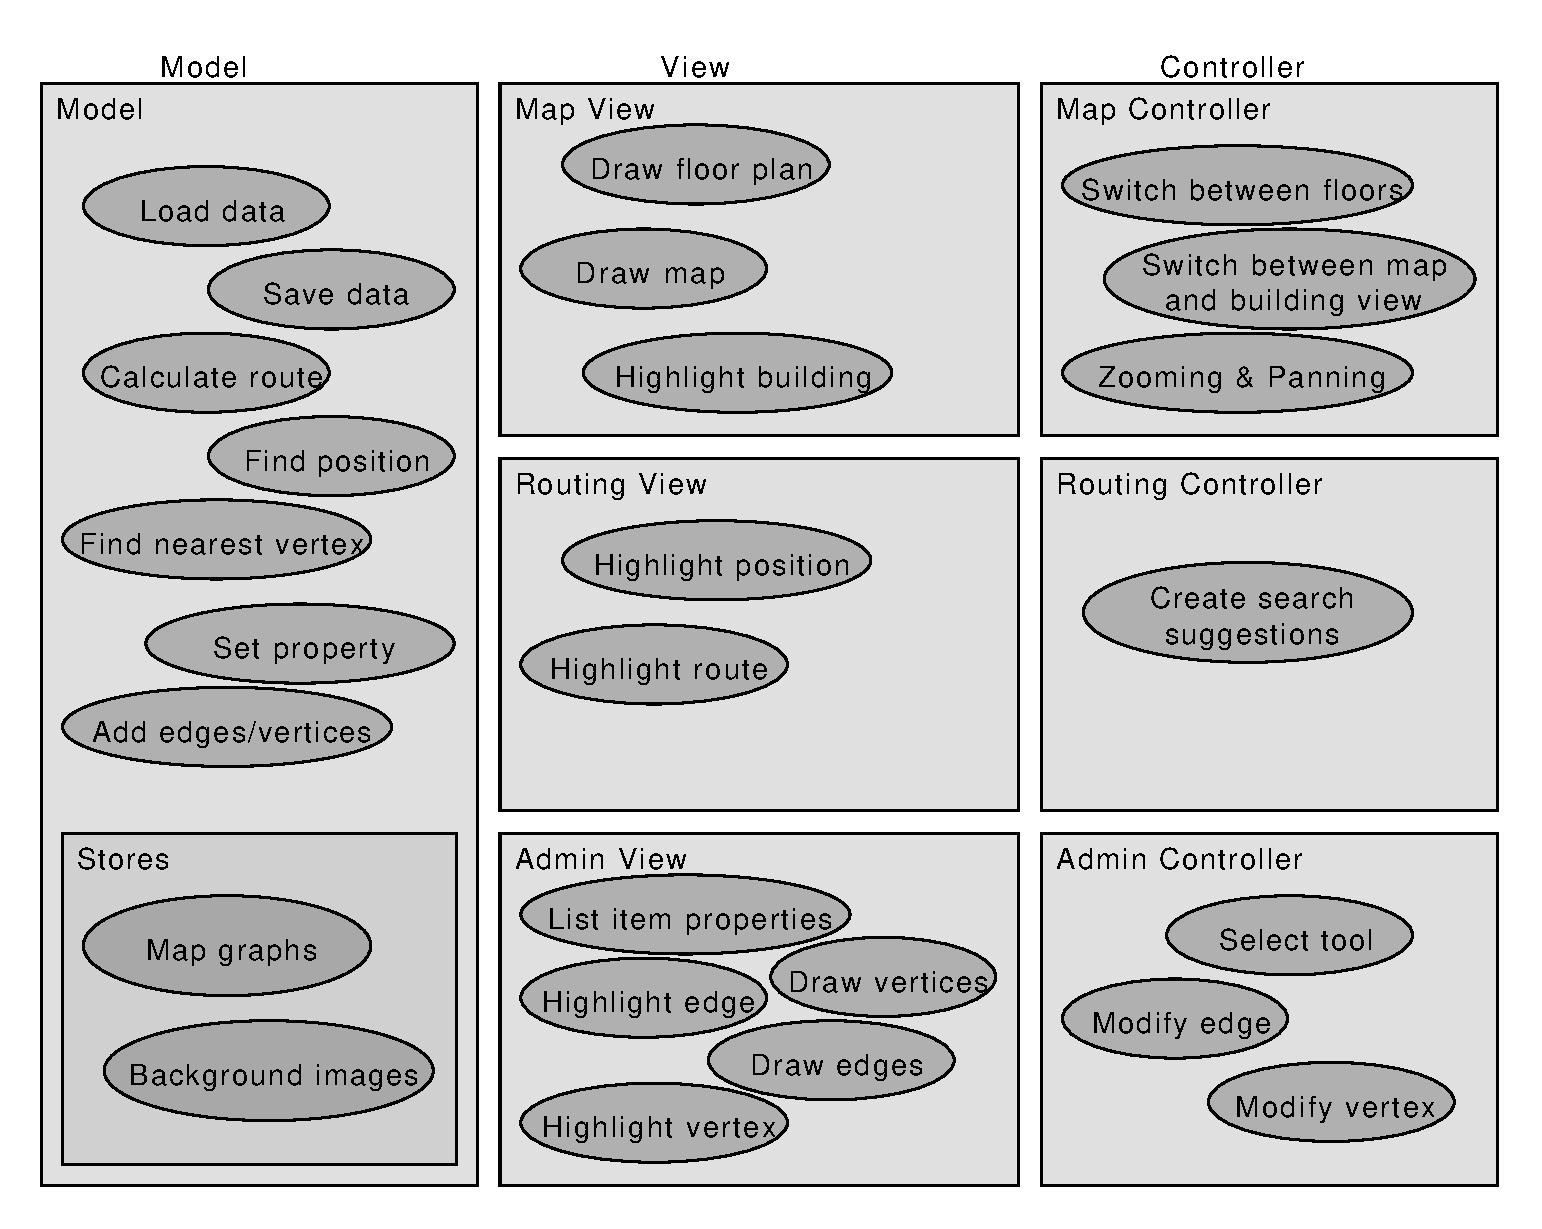
\includegraphics[scale=0.5]{diagrams/mvc.pdf}
	\caption{The parts of the application in the MVC-Architecture}
\end{figure}

The \textit{MVC-architecture} is applied three times inside the project: The map component, the routing tool and the administration tool all use separate views and controllers but share the same model. However, since the routing tool and the administration tool both need to work with the map, they extend the map view and the map controller. \\*
The model has to do the work of the program. It stores the opened \textit{routing graph} and the image that should be displayed as background of the \textit{map} for the exterior and every building floor. It also does the actual routing inside the \textit{routing graph} and offers some functions like finding the nearest vertex for a position. \\*
The view of the map component has to display the currently loaded \textit{map}. This \textit{map} consists of the \textit{background image} either for an interior or an exterior \textit{map}. When the exterior \textit{map} is displayed, a building might be highlighted if one is selected. The routing and administration tools extend this \textit{map} view with their own functionality, for example the routing tool needs a way to display the calculated routes. The administration view shows besides the \textit{map} a panel with the \textit{properties} of the selected edge or vertex.\\*
The controller has to handle the user input. In the case of the map component this means panning and zooming of the \textit{map}, as well as switching between exterior and interior. The controller of the routing tool supports the user to enter his destination since it compares the input with the names of all locations and creates a list of search suggestions. The administration tool controller mainly parses the user input and passes it on to the model to modify the \textit{routing graph}.

\subsection{Use Case Diagram}

\begin{figure}[h]
	\centering
	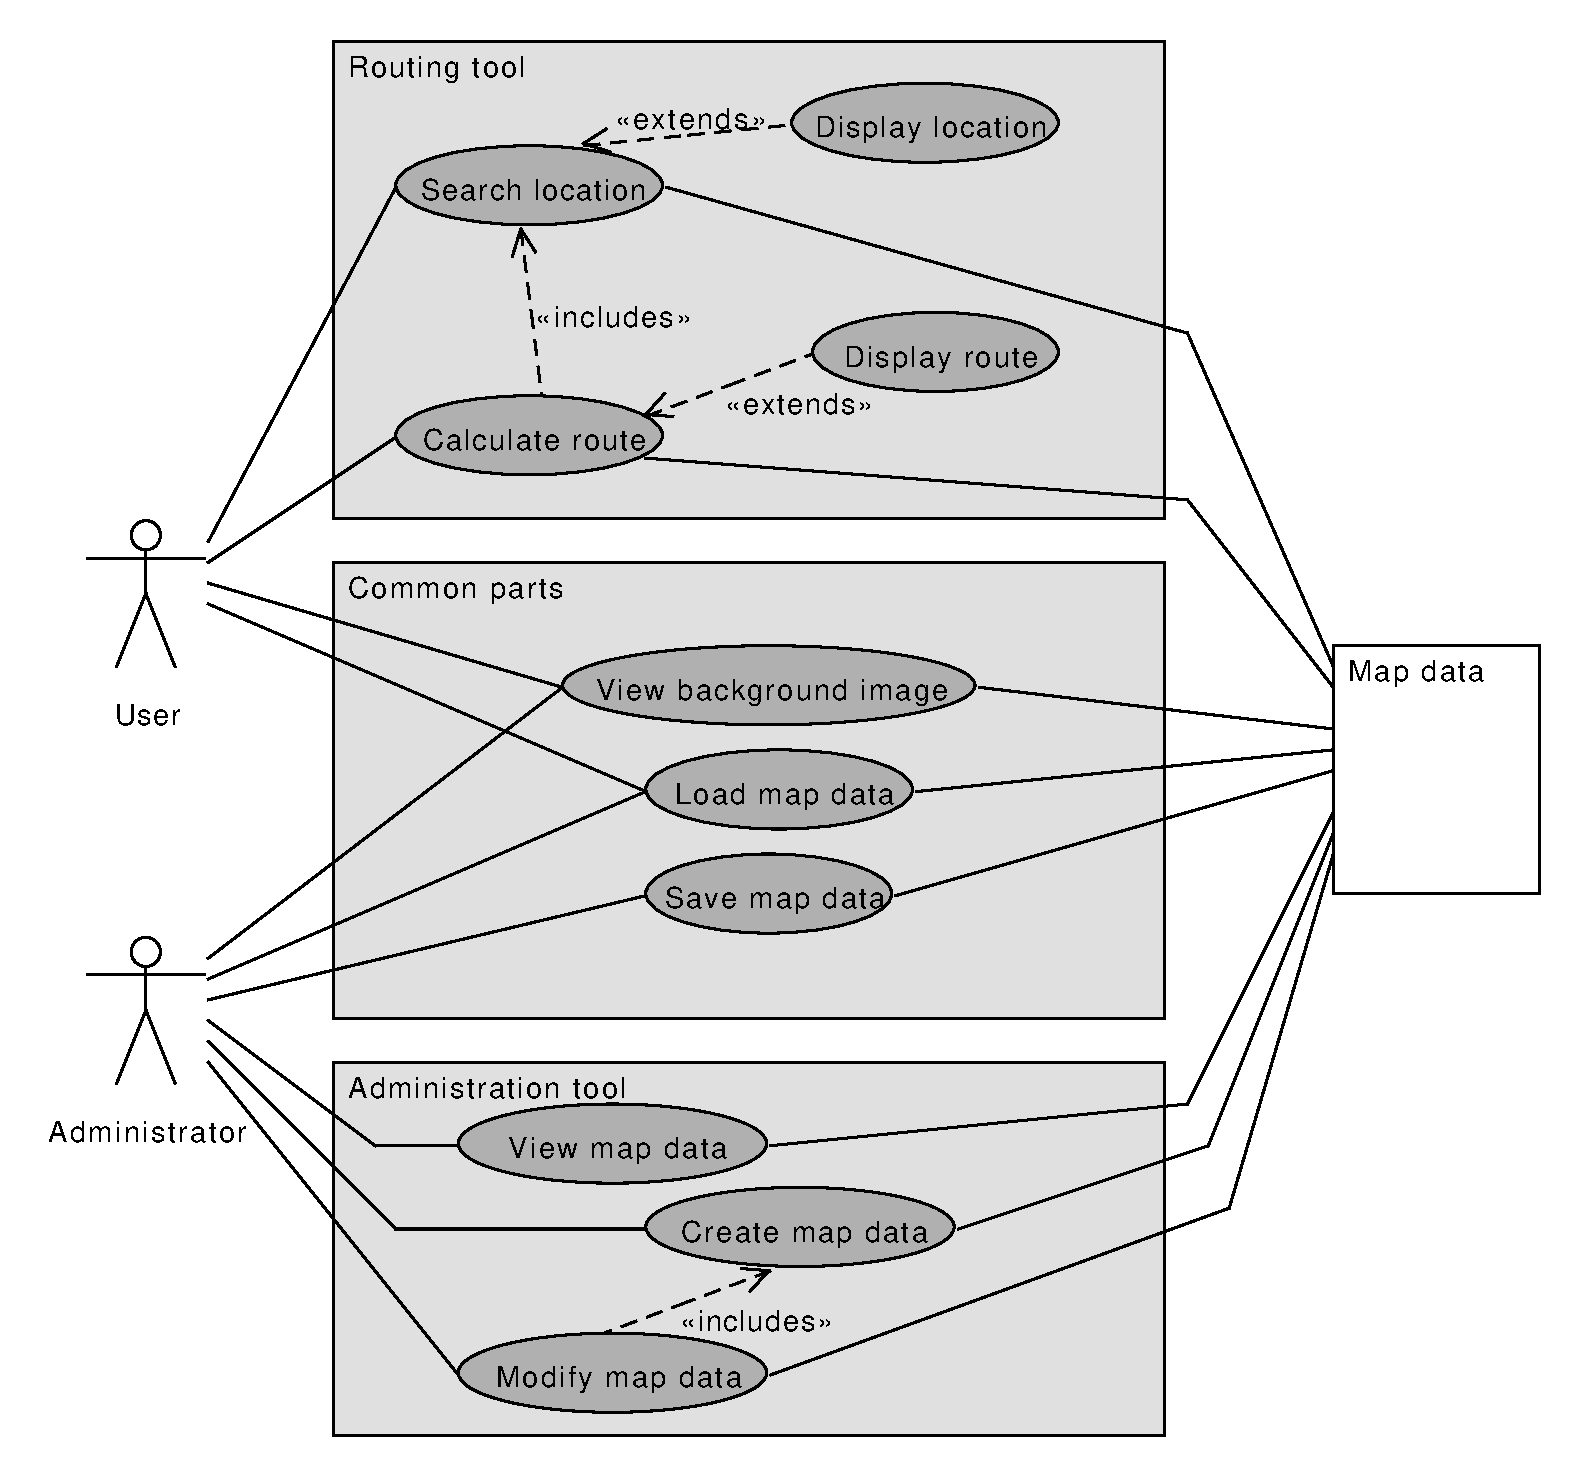
\includegraphics[scale=0.5]{diagrams/usecase.pdf}
	\caption{Possible use-cases of the program}
\end{figure}

After starting the routing tool and loading the \textit{map}, a zoomed out view of the area is displayed. Now the user can look at the \textit{background image} without entering positions. It is possible to zoom into the \textit{map}, move the displayed section and click on buildings to show their floor plan maps. \\*
If he wants to, he can enter a position. This position can be given as coordinates, address, the name of a place or by clicking on the wanted position. By entering only one position, the position will be displayed at the \textit{map} but when he inputs a second position a route between the locations can be calculated and is displayed. The search criteria can be further specified by filtering for some \textit{properties}, for example only stair-free routes can be allowed. \\

To provide this functionality, both program parts needs to have access to the map. This data consists of the \textit{routing graph} that can be modified with the administration tool and the \textit{background image} which has been provided by the user and is linked to the \textit{routing graph}.

\subsection{Activitiy Diagrams}

\subsubsection*{Routing Tool}

\begin{figure}[h]
	\centering
	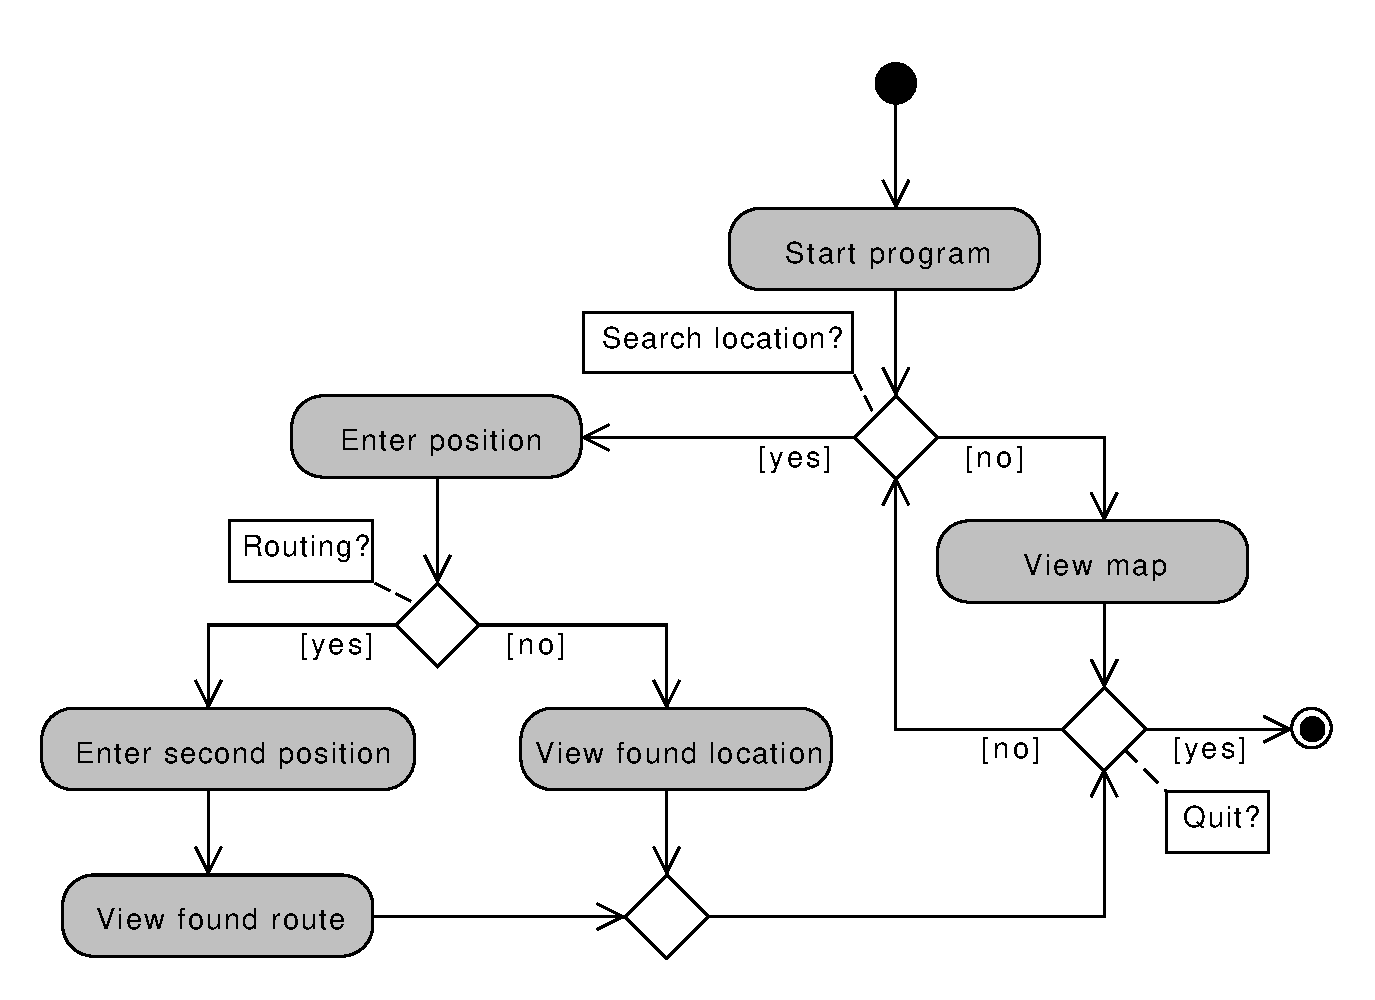
\includegraphics[scale=0.5]{diagrams/activity_routing.pdf}
	\caption{A possible work-flow when using the routing tool}
\end{figure}

The routing tool can be used in three different ways: The user can look at the map, he can search for a location and he can calculate a route between two positions. When he enters a position, the program displays it. After a second position has been entered, the program displays a route between the positions, if one could be found. While calculating this route, the program will follow the restrictions defined by the selected filters. When the user is finished with looking at his route or location, he can either enter new positions or exit the program.

\subsubsection*{Administration Tool}

\begin{figure}[h]
	\centering
	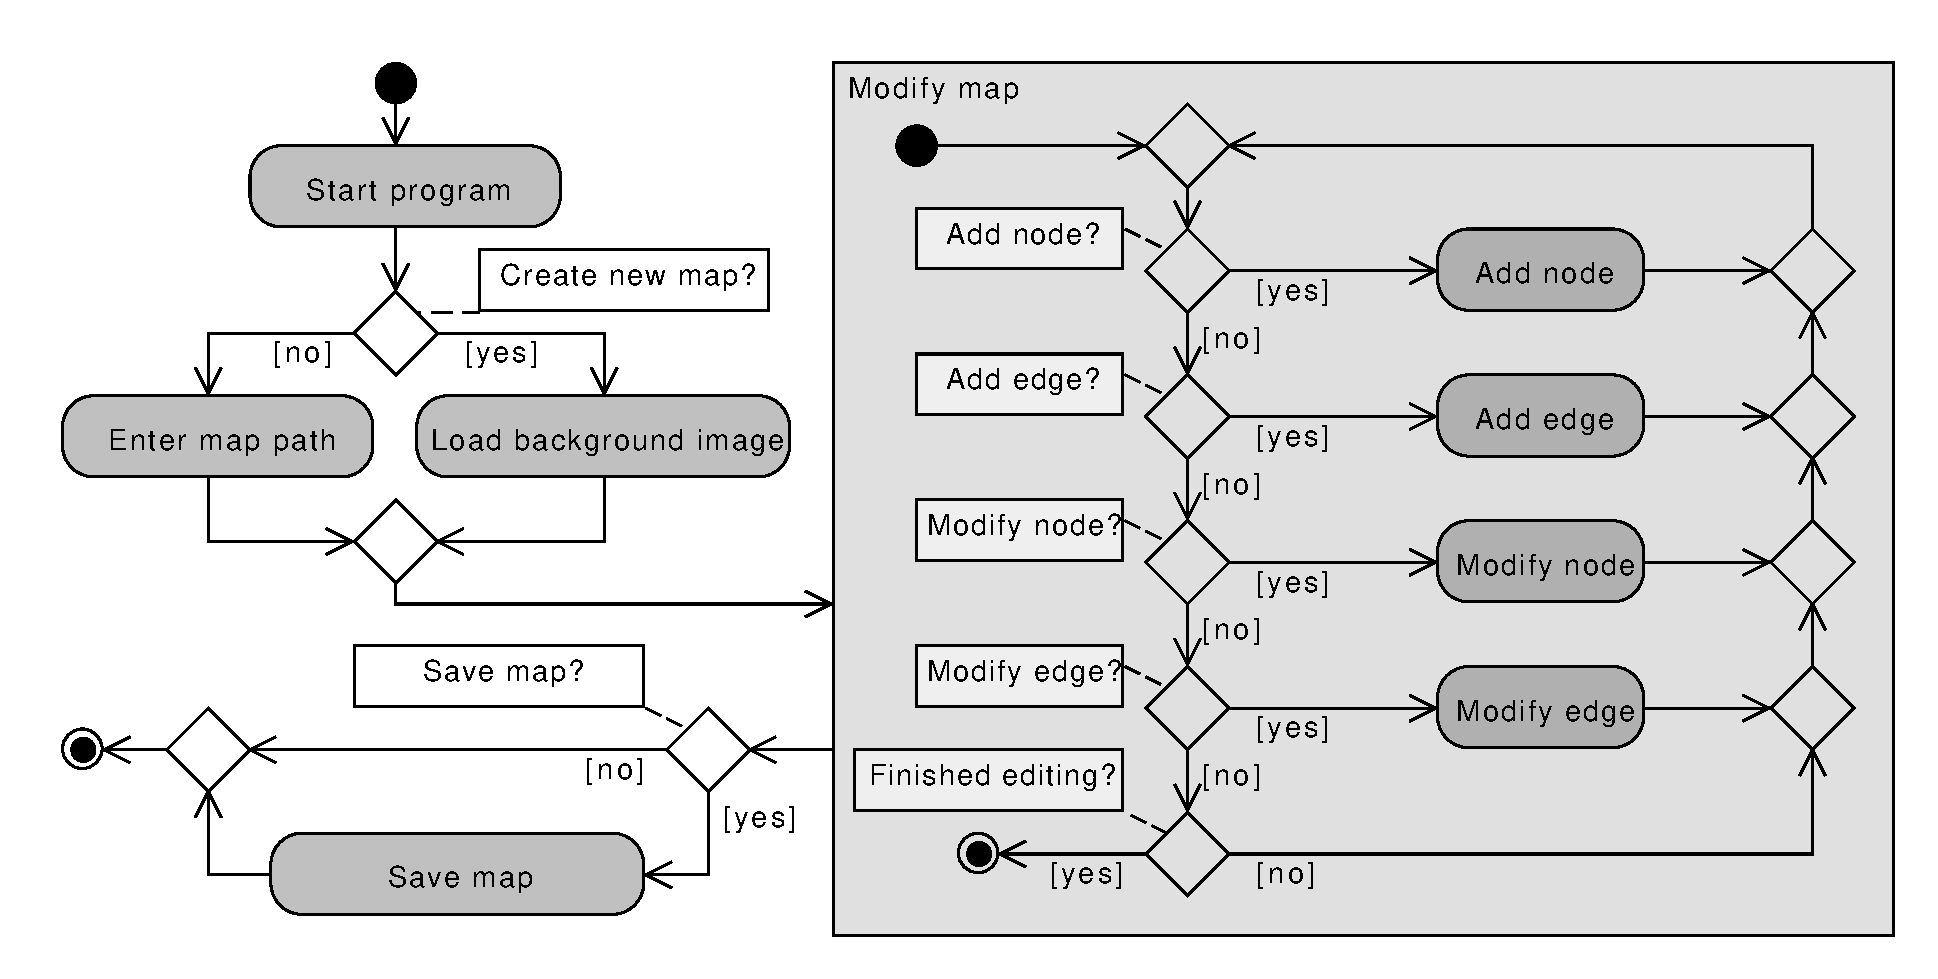
\includegraphics[scale=0.5]{diagrams/activity_admin.pdf}
	\caption{A possible work-flow when using the administration tool}
\end{figure}

The first decision after starting the editor is whether to load an existing map or to load a \textit{background image} to create a new \textit{map}. After doing one of these, the \textit{map} can be modified. To do this the user can add, edit or remove nodes or edges. The \textit{properties} of existing nodes and edges can be edited to attach further information to them, e.g. adding the name of a building to a node. When the user has finished editing the \textit{map}, he can save his changes or drop them if they are not useful.
